\documentclass[conference]{IEEEtran}
\IEEEoverridecommandlockouts
\usepackage{cite}
\usepackage{amsmath,amssymb,amsfonts}
\usepackage{graphicx}
\usepackage{booktabs}
\usepackage{multirow}
\usepackage{xcolor}
\usepackage{tikz}
\usetikzlibrary{positioning,arrows.meta,calc}
\usepackage[hidelinks]{hyperref}
\newcommand{\ablDropAugnojitter}{0.36}
\newcommand{\ablDropAugnone}{-0.45}
\newcommand{\ablDropNoattn}{-0.68}
\newcommand{\ablDropNogate}{-1.39}
\newcommand{\ablDropNomotion}{-1.45}
\newcommand{\ablDropNotemporal}{-0.48}
\newcommand{\ablDropXyz}{-0.20}
\newcommand{\ablMpDropNoattn}{2.92}
\newcommand{\ablMpDropNomotion}{-4.10}
\newcommand{\ablMpDropNotemporal}{8.25}
\newcommand{\ablSeeds}{two}
\newcommand{\auditSelConsistent}{91}
\newcommand{\auditSelRuns}{91}
\newcommand{\miCiHi}{51.58}
\newcommand{\miCiLo}{48.33}
\newcommand{\mipointnetTwoAcc}{8.07}
\newcommand{\mipointnetTwoFone}{5.12}
\newcommand{\mipointnetTwoStd}{5.47}
\newcommand{\mipointnetTwoTopthree}{21.44}
\newcommand{\mipointnetAcc}{32.57}
\newcommand{\mipointnetFone}{29.72}
\newcommand{\mipointnetStd}{4.59}
\newcommand{\mipointnetTopthree}{59.50}
\newcommand{\mipointnetlstmAcc}{28.11}
\newcommand{\mipointnetlstmFone}{28.09}
\newcommand{\mipointnetlstmStd}{4.06}
\newcommand{\mipointnetlstmTopthree}{56.08}
\newcommand{\mipointnetrobustAcc}{18.66}
\newcommand{\mipointnetrobustFone}{15.67}
\newcommand{\mipointnetrobustStd}{8.83}
\newcommand{\mipointnetrobustTopthree}{40.90}
\newcommand{\mistptliteAcc}{45.79}
\newcommand{\mistptliteFone}{45.95}
\newcommand{\mistptliteStd}{6.30}
\newcommand{\mistptliteTopthree}{73.90}
\newcommand{\mistptlitekdAcc}{48.55}
\newcommand{\mistptlitekdFone}{47.62}
\newcommand{\mistptlitekdStd}{4.35}
\newcommand{\mistptlitekdTopthree}{76.35}
\newcommand{\mistptlitekdrobustAcc}{49.56}
\newcommand{\mistptlitekdrobustFone}{48.80}
\newcommand{\mistptlitekdrobustStd}{1.98}
\newcommand{\mistptlitekdrobustTopthree}{78.03}
\newcommand{\mistptteacherAcc}{50.39}
\newcommand{\mistptteacherFone}{50.84}
\newcommand{\mistptteacherStd}{1.39}
\newcommand{\mistptteacherTopthree}{75.81}
\newcommand{\mpAuditLeakFrames}{72.9}
\newcommand{\mpAuditLeakOverlap}{58.7}
\newcommand{\mpAuditLeakWins}{91.2}
\newcommand{\mpOfficialAcc}{58.38}
\newcommand{\mpOursAcc}{49.56}
\newcommand{\mpOursFone}{48.80}
\newcommand{\mpOursIntAcc}{49.59}
\newcommand{\mpOursStd}{1.98}
\newcommand{\mpOursTopthree}{78.03}
\newcommand{\mpRandomAcc}{79.48}
\newcommand{\mpRandomPnAcc}{44.44}
\newcommand{\mpSubjPntwoAcc}{8.07}
\newcommand{\oursFpMB}{0.49}
\newcommand{\oursIntMB}{0.14}
\newcommand{\oursLat}{2.58}
\newcommand{\oursMflops}{36.6}
\newcommand{\oursParamsK}{117.5}
\newcommand{\raCiHi}{97.62}
\newcommand{\raCiLo}{96.52}
\newcommand{\radgcnnAcc}{95.85}
\newcommand{\radgcnnFone}{95.89}
\newcommand{\radgcnnStd}{0.00}
\newcommand{\radgcnnTopthree}{99.86}
\newcommand{\rapointnetTwoAcc}{97.34}
\newcommand{\rapointnetTwoFone}{97.37}
\newcommand{\rapointnetTwoStd}{0.18}
\newcommand{\rapointnetTwoTopthree}{99.66}
\newcommand{\rapointnetAcc}{96.31}
\newcommand{\rapointnetFone}{96.36}
\newcommand{\rapointnetStd}{0.66}
\newcommand{\rapointnetTopthree}{99.73}
\newcommand{\rapointnetlstmAcc}{96.14}
\newcommand{\rapointnetlstmFone}{96.16}
\newcommand{\rapointnetlstmStd}{0.23}
\newcommand{\rapointnetlstmTopthree}{99.57}
\newcommand{\rapointnetrobustAcc}{97.38}
\newcommand{\rapointnetrobustFone}{97.40}
\newcommand{\rapointnetrobustStd}{0.11}
\newcommand{\rapointnetrobustTopthree}{99.64}
\newcommand{\rapointtransformerAcc}{97.01}
\newcommand{\rapointtransformerFone}{97.04}
\newcommand{\rapointtransformerStd}{0.25}
\newcommand{\rapointtransformerTopthree}{99.86}
\newcommand{\rastptliteAcc}{96.22}
\newcommand{\rastptliteFone}{96.27}
\newcommand{\rastptliteStd}{1.43}
\newcommand{\rastptliteTopthree}{99.67}
\newcommand{\rastptlitekdAcc}{96.04}
\newcommand{\rastptlitekdFone}{96.08}
\newcommand{\rastptlitekdStd}{0.78}
\newcommand{\rastptlitekdTopthree}{99.57}
\newcommand{\rastptlitekdrobustAcc}{96.83}
\newcommand{\rastptlitekdrobustFone}{96.88}
\newcommand{\rastptlitekdrobustStd}{0.69}
\newcommand{\rastptlitekdrobustTopthree}{99.71}
\newcommand{\rastptteacherAcc}{96.44}
\newcommand{\rastptteacherFone}{96.48}
\newcommand{\rastptteacherStd}{1.43}
\newcommand{\rastptteacherTopthree}{99.54}
\newcommand{\rastpttinykdAcc}{96.86}
\newcommand{\rastpttinykdFone}{96.90}
\newcommand{\rastpttinykdStd}{0.17}
\newcommand{\rastpttinykdTopthree}{99.66}
\newcommand{\ravoxeltdcnnAcc}{95.01}
\newcommand{\ravoxeltdcnnFone}{95.03}
\newcommand{\ravoxeltdcnnStd}{0.16}
\newcommand{\ravoxeltdcnnTopthree}{99.68}
\newcommand{\rhOursAcc}{96.83}
\newcommand{\rhOursFone}{96.88}
\newcommand{\rhOursIntAcc}{96.82}
\newcommand{\rhOursStd}{0.69}
\newcommand{\silPointNet}{0.24}
\newcommand{\silSTPTLiteKDrobust}{0.82}
\newcommand{\trrhablxyz}{96.42}
\newcommand{\trrhxyzmpinitfFull}{95.23}
\newcommand{\trrhxyzmpinitfQuarter}{87.45}
\newcommand{\trrhxyzmpinitfTen}{78.98}
\newcommand{\trrhxyzscratchfQuarter}{86.10}
\newcommand{\trrhxyzscratchfTen}{61.22}
\newcommand{\xaiCorr}{0.49}


\begin{document}

\title{Privacy-Preserving Human Activity Recognition from mmWave Radar Point Clouds using Lightweight Point Transformers}

\author{
\IEEEauthorblockN{Abarajitha S K, G Aswath Rupan, Indu Vadana M D, Murugan S}
\IEEEauthorblockA{Department of Information Technology, PSG College of Technology, Coimbatore, India\\
\{23i301, 23i321, 23i323, 23i338\}@psgtech.ac.in}
}

\maketitle

\begin{abstract}
Millimetre-wave (mmWave) radar can recognise human activities without capturing
images of people. Its point clouds, however, are extremely sparse and full of
clutter, and the accuracies reported for them depend heavily on how the data are
split. We present \emph{STPT-Lite}, a lightweight spatio-temporal point
transformer that applies self-attention among the points of short temporal
segments and then across segment tokens. Each token is enriched with an explicit
radar motion descriptor, and the model needs neither farthest-point sampling nor
$k$-NN search. Doppler-based person centring and spatial gating remove the static
clutter that makes up about half of the radar returns. With knowledge
distillation from a larger teacher, noise-robust training and INT8 weights, STPT-Lite has
\oursParamsK\,K parameters, needs \oursMflops\,MFLOPs per 2-s window, occupies
\oursIntMB\,MB and runs in \oursLat\,ms on one CPU thread. We evaluate it against
six re-implemented baselines (voxel CNN-LSTM, PointNet, PointNet+BiLSTM,
PointNet++, DGCNN and Point Transformer) on two public datasets with three seeds
and leakage-free splits. STPT-Lite reaches \rhOursAcc\,$\pm$\,\rhOursStd\% on the
official RadHAR test recordings and \mpOursAcc\,$\pm$\,\mpOursStd\% top-1
(\mpOursTopthree\% top-3) on 49 MiliPoint actions performed by subjects never
seen in training, against \mipointnetAcc\% for the best baseline. Under a random
window split, which is leaky, the same architecture scores \mpRandomAcc\%, showing how strongly the evaluation protocol inflates
reported accuracy. Ablations, cross-dataset transfer, robustness tests and
attention/occlusion analyses explain where the accuracy comes from.
\end{abstract}

\begin{IEEEkeywords}
mmWave radar, point clouds, human activity recognition, privacy-preserving sensing, point transformer, knowledge distillation, edge AI
\end{IEEEkeywords}

\section{Introduction}
Monitoring daily activity at home, for example in elderly care, fall-risk
screening or rehabilitation, needs sensing that works in the dark, through
clothing, and without recording images of people. Cameras fail the last
requirement, and wearables depend on users remembering to wear and charge them.
Low-cost single-chip mmWave radars (60--81\,GHz) output a sparse 3-D point cloud
with a Doppler velocity for every point. Identity is not visually recoverable
from such data, which makes radar attractive for privacy-preserving human
activity recognition (HAR) \cite{singh2019radhar,ullmann2023survey}.

Radar point clouds differ sharply from the LiDAR and CAD data that most
point-cloud networks are designed for. A frame contains only about 6--21 returns
(Section~\ref{sec:data}). Many returns are static clutter or multipath rather than
the person. The useful signal lies in how the cloud moves over time rather than
in its instantaneous shape. Existing approaches either voxelise the
cloud \cite{singh2019radhar}, which wastes computation on empty cells, or apply
dense-point backbones such as PointNet++, DGCNN or Point Transformer
\cite{qi2017pointnet2,wang2019dgcnn,zhao2021pt}. Those backbones rely on
farthest-point sampling and $k$-NN search, which are slow on embedded processors.
A second, less visible problem concerns evaluation. Radar HAR samples are short
windows cut with large overlap from long recordings, so random window-level
splits place near-identical samples in training and test. Published accuracies
on the same dataset consequently range from about 34\% to 98\%
\cite{cui2023milipoint,zakka2025makgcn}.

This paper studies privacy-preserving HAR from mmWave point clouds with a focus
on two things: models that are light enough for edge deployment, and
measurements that are honest. Our contributions are:
\begin{itemize}
\item \textbf{STPT-Lite}, a factorised spatio-temporal point transformer.
  Attention runs within short temporal segments and then across segment tokens,
  each token is augmented with an explicit radar motion descriptor, and no FPS or
  $k$-NN is needed. With knowledge distillation, noise-robust training and INT8
  weights it reaches
  \rhOursAcc\% on RadHAR with \oursParamsK\,K parameters, \oursMflops\,MFLOPs,
  \oursIntMB\,MB of storage and \oursLat\,ms single-thread CPU latency.
\item \textbf{Radar-specific pre-processing}: moving-point (Doppler-based) person
  centring and spatial gating. Together they remove the static clutter that makes
  up about half of the returns, along with the scene shortcut that clutter
  creates.
\item \textbf{Leakage-free evaluation} on two public datasets: recording-disjoint
  validation on RadHAR and a subject-disjoint split on MiliPoint, where STPT-Lite
  reaches \mpOursAcc\% top-1 on 49 actions performed by unseen people. The same
  architecture scores \mpRandomAcc\% under a leaky random split, which quantifies how
  much the protocol inflates reported accuracy.
\item A study with \textbf{six re-implemented baselines, three seeds, paired
  significance tests, ablations, MiliPoint$\rightarrow$RadHAR transfer,
  robustness to seven controlled perturbation types, and explainability} (temporal attention,
  occlusion and point saliency).
\end{itemize}
Code, pre-processing and all run logs are released for reproducibility.

\section{Related Work}
\label{sec:related}

\textbf{mmWave point-cloud HAR.} RadHAR \cite{singh2019radhar} released the
MMActivity data used here. It voxelised each frame into a $10\times32\times32$
grid and classified sequences with a time-distributed CNN and a BiLSTM (90.47\%
accuracy). Later work moved to models that consume points directly.
MMPoint-GNN \cite{gong2021mmpointgnn} builds dynamic graphs per frame. Lee and
Kim \cite{lee2022gnn} pre-train a GNN on 3-D joint coordinates and report
96.55\% on RadHAR. Gu et al.\ \cite{gu2024lpn} pair a light PointNet with a
bidirectional linear-attention LSTM (95.12\%, 79.7\,K parameters).
MAK-GCN \cite{zakka2025makgcn} learns multi-head adaptive graph kernels (97.54\%,
1.86\,M parameters). OG-PCL \cite{yan2025ogpcl} uses occupancy-gated
convolutions (91.75\%, 0.83\,M parameters) and reports PCT+LSTM
\cite{guo2021pct} at 92.78\%. Gao et al.\ \cite{gao2025star} model each frame as
a star graph around a virtual centre. Lim et al.\ \cite{lim2024fpga} deploy a
4-bit pillar-based classifier on an FPGA. For gestures, Pantomime
\cite{palipana2021pantomime} and Tesla-Rapture \cite{salami2023tesla} showed
that sparse radar point clouds support lightweight recognisers. The same sensing
also drives rehabilitation \cite{an2021mars}, mesh reconstruction
\cite{xue2021mmmesh,chen2022mmbody} and scene flow \cite{ding2024milliflow}.
Ullmann et al.\ \cite{ullmann2023survey} survey radar-based continuous HAR.

\textbf{Benchmarks and evaluation protocols.} MiliPoint \cite{cui2023milipoint}
(49 actions, 11 subjects) and MM-Fi \cite{yang2023mmfi} are recent large-scale
benchmarks. On MiliPoint action classification the original authors report at most
34.45\% (PointNet++), whereas MAK-GCN reports 98.25\% under an
80/10/10 split. Several RadHAR studies validate on 20\% of training windows drawn at
random, and those windows overlap by 50 of 60 frames. Data leakage of this kind is a
known way to inflate results \cite{kaufman2012leakage}. To our knowledge, no
prior work has measured its effect on radar point-cloud HAR.

\textbf{Point-cloud backbones.} PointNet \cite{qi2017pointnet} and PointNet++
\cite{qi2017pointnet2} introduced learning on raw point sets. DGCNN
\cite{wang2019dgcnn} builds dynamic $k$-NN graphs. Point Transformer
\cite{zhao2021pt}, PCT \cite{guo2021pct}, PTv2/PTv3 \cite{wu2022ptv2,wu2024ptv3},
PointNeXt \cite{qian2022pointnext} and PointMLP \cite{ma2022pointmlp} raised accuracy
on dense LiDAR and CAD data. P4Transformer \cite{fan2021p4t} handles point-cloud
videos. All of these assume hundreds to thousands of points per frame and rely on
FPS and $k$-NN, which are costly on micro-controllers.

\textbf{Research gap.} (i) Most radar HAR models either reuse dense-point
backbones or voxelise the data. Few exploit what is specific to radar: extreme
sparsity, a direct Doppler measurement, and static clutter. (ii) Reported
accuracies are rarely obtained with leakage-free (recording- or subject-disjoint)
splits, and protocols differ between papers. (iii) Cross-dataset transfer
between radar datasets and edge cost (latency, size, quantisation) are seldom
reported together. This work addresses all three gaps.

\section{Methodology}
\label{sec:method}

\subsection{Problem formulation}
A frequency-modulated continuous-wave (FMCW) mmWave radar outputs, at every
frame $t$, a small unordered set of detections
$\mathcal{F}_t=\{\mathbf{p}_{t,i}\}_{i=1}^{n_t}$ with
$\mathbf{p}=(x,y,z,v,\iota)$: the 3-D position, the radial (Doppler) velocity $v$
and the reflected intensity $\iota$. The count $n_t$ is small and varies
(median 21 on RadHAR and 6 on MiliPoint, Section~\ref{sec:data}). Given a
window $\mathcal{W}=(\mathcal{F}_{t_0},\dots,\mathcal{F}_{t_0+T-1})$ of $T$ frames
(2\,s), we learn $f_\theta:\mathcal{W}\mapsto\hat{y}\in\{1,\dots,K\}$ that
predicts the activity. $f_\theta$ must be invariant to the order of points within
a frame, robust to missing detections, and cheap enough to run on an edge device
at the radar frame rate. The radar never records an image of the person, so the
sensing is privacy-preserving by construction.

\subsection{Radar-specific pre-processing}
\label{sec:preproc}
Raw RadHAR windows contain three kinds of returns (Fig.~\ref{fig:preproc}):
antenna self-returns at $x\approx0$, static multipath and clutter several metres
behind the subject, and the person. We apply three steps.
\textbf{(i) ROI}: drop returns with $x<0.3$\,m (34.6\% of all points).
\textbf{(ii) Person centring}: the window centre $\mathbf{c}$ is the median
position of the \emph{moving} returns ($v\neq0$), because static clutter has
zero radial velocity; if a window has no moving return we fall back to the median of
all returns. Coordinates are expressed relative to $\mathbf{c}$, which removes
the subject's absolute position and distance from the radar.
\textbf{(iii) Spatial gating}: returns farther than $r_g=1.2$\,m (horizontally)
from $\mathbf{c}$ are discarded. This removes on average 50.1\% of the remaining
returns, almost all of them static clutter. Gating also removes a shortcut: the
same furniture appears in training and test recordings, so a model could use
the clutter to recognise the scene instead of the motion.
MiliPoint is already cropped to the subject and has no Doppler channel, so only
median centring is applied. Its axes are remapped to the RadHAR convention ($x$
forward, $y$ lateral, $z$ up) so that both datasets share one coordinate frame.

\begin{figure}[t]
\centering
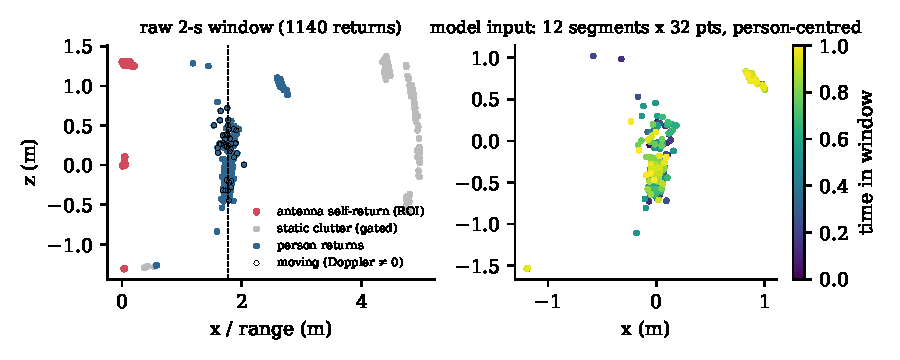
\includegraphics[width=\columnwidth]{../figures/preproc_before_after.pdf}
\caption{A raw 2-s RadHAR window (left): antenna self-returns (red), static
clutter removed by gating (grey), person returns (blue) and moving returns
(circled). Right: the resulting person-centred model input, coloured by time.}
\label{fig:preproc}
\end{figure}

\textbf{Temporal segmentation and sampling.} A window is split into $G=12$
equal segments (5 frames on RadHAR at 30\,Hz and 4 frames on MiliPoint at 24\,Hz).
From each segment we sample $P=32$ returns, with replacement when fewer exist.
This gives a fixed tensor $\mathbf{X}\in\mathbb{R}^{G\times P\times C}$ with
$C=6$ features: centred $x,y,z$; $v$; $\iota$ standardised with training
statistics; and the normalised time inside the window. A mask
$\mathbf{M}\in\{0,1\}^{G\times P}$ marks empty segments. Accumulating a few
frames per segment counters the extreme sparsity of single frames while keeping
temporal order across segments.

\textbf{Augmentation (training only).} Random rotation about the vertical axis
($\pm15^\circ$), isotropic scaling ($[0.9,1.1]$), Gaussian jitter
($\sigma=1$\,cm) and fresh random point sampling at every epoch.

\begin{figure*}[t]
\centering
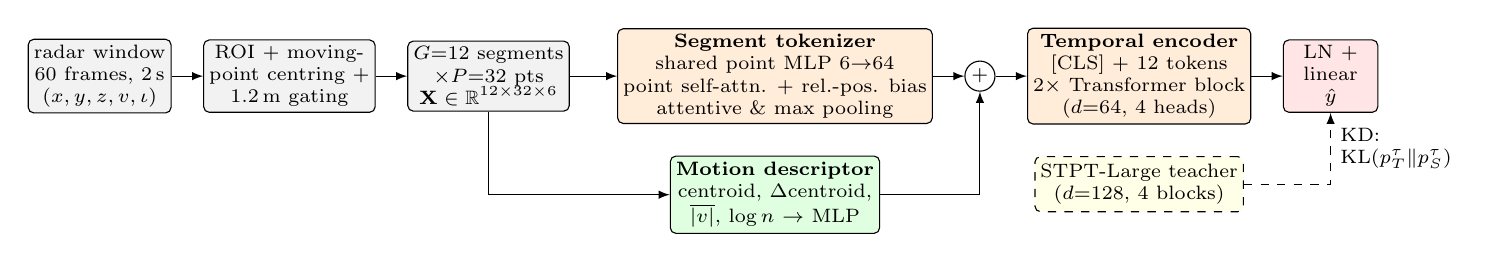
\begin{tikzpicture}[
  font=\scriptsize, >=latex,
  box/.style={draw, rounded corners=2pt, align=center, minimum height=7mm, inner sep=2pt},
  frozen/.style={box, fill=blue!8},
  train/.style={box, fill=orange!15},
  mot/.style={box, fill=green!12},
  ]
\node[box, fill=gray!10, minimum width=17mm] (in) {radar window\\$60$ frames, $2$\,s\\$(x,y,z,v,\iota)$};
\node[box, right=4mm of in, minimum width=19mm, fill=gray!10] (pre) {ROI + moving-\\point centring +\\$1.2$\,m gating};
\node[box, right=4mm of pre, minimum width=16mm, fill=gray!10] (seg) {$G{=}12$ segments\\$\times P{=}32$ pts\\$\mathbf{X}\in\mathbb{R}^{12\times32\times6}$};
\node[train, right=6mm of seg, minimum width=26mm] (tok) {\textbf{Segment tokenizer}\\shared point MLP $6{\to}64$\\point self-attn. + rel.-pos. bias\\attentive \& max pooling};
\node[mot, below=4mm of tok, minimum width=26mm] (md) {\textbf{Motion descriptor}\\centroid, $\Delta$centroid,\\$\overline{|v|}$, $\log n$ $\to$ MLP};
\node[circle, draw, right=4mm of tok, inner sep=1pt] (plus) {$+$};
\node[train, right=4mm of plus, minimum width=24mm] (tem) {\textbf{Temporal encoder}\\$[\mathrm{CLS}]$ + 12 tokens\\$2\times$ Transformer block\\($d{=}64$, 4 heads)};
\node[box, right=4mm of tem, minimum width=12mm, fill=red!10] (out) {LN +\\linear\\$\hat{y}$};
\draw[->] (in) -- (pre); \draw[->] (pre) -- (seg); \draw[->] (seg) -- (tok);
\draw[->] (seg.south) |- (md.west); \draw[->] (tok) -- (plus); \draw[->] (md.east) -| (plus.south);
\draw[->] (plus) -- (tem); \draw[->] (tem) -- (out);
\node[box, dashed, below=4mm of tem, minimum width=24mm, fill=yellow!10] (teach) {STPT-Large teacher\\($d{=}128$, 4 blocks)};
\draw[->, dashed] (teach.east) -| node[pos=0.75, right, align=left]{KD:\\$\mathrm{KL}(p_T^{\tau}\Vert p_S^{\tau})$} (out.south);
\end{tikzpicture}
\caption{STPT-Lite. Points are attended to only \emph{within} a short temporal
segment (cost $O(GP^2)$), each segment is compressed into one token enriched
with an explicit radar motion descriptor, and a small Transformer attends
\emph{across} the $G$ segment tokens ($O(G^2)$). No farthest-point sampling or
$k$-NN search is needed. A larger STPT teacher is distilled into the student,
whose weights are finally quantised to INT8.}
\label{fig:arch}
\end{figure*}

\subsection{STPT-Lite: a factorised spatio-temporal point transformer}
Generic point-cloud backbones (PointNet++, DGCNN, Point Transformer) treat the
accumulated window as one static set. They spend most of their computation on
farthest-point sampling and $k$-NN neighbourhoods over the whole set, and they
encode time only as one more coordinate. Radar HAR has the opposite structure:
very few points per instant, but strong regularity over time. STPT-Lite
(Fig.~\ref{fig:arch}) therefore factorises attention into a spatial part and a
temporal part.

\textbf{Segment tokenizer.} A shared MLP embeds every point,
$\mathbf{h}=\phi(\mathbf{x})\in\mathbb{R}^{d}$ ($d=64$). One pre-norm
multi-head self-attention block then runs over the $P$ points of each segment,
with a learned relative-position bias computed from pairwise 3-D offsets:
\begin{equation}
\mathbf{A}^{(h)}_{ij}=\operatorname{softmax}_j\!\Big(\tfrac{\mathbf{q}_i^{(h)}\cdot\mathbf{k}_j^{(h)}}{\sqrt{d/H}}+\beta^{(h)}(\mathbf{x}_i^{xyz}-\mathbf{x}_j^{xyz})+\log m_j\Big),
\end{equation}
where $\beta$ is a two-layer MLP $\mathbb{R}^3\!\to\!\mathbb{R}^{H}$ and $m_j$
is the mask. The block is followed by a feed-forward layer. The segment token
concatenates attentive pooling,
$\mathbf{a}=\sum_i\operatorname{softmax}_i(\mathbf{w}^\top\mathbf{h}_i)\mathbf{h}_i$,
with max pooling, and projects the result back to $d$ dimensions. Because $P=32$,
full attention inside a segment costs only $G\cdot P^2=12{,}288$ pairs, against
$(GP)^2\approx1.5\times10^5$ for joint attention over the window.

\textbf{Motion descriptor.} Radar measures motion directly, so we give it to the
model explicitly. For each segment $g$ we compute
$\mathbf{u}_g=[\bar{\mathbf{x}}_g,\;\bar{\mathbf{x}}_g-\bar{\mathbf{x}}_{g-1},\;\overline{|v|}_g,\;\log(1+n_g)]\in\mathbb{R}^8$,
i.e.\ the segment centroid, its displacement since the previous segment, the
mean Doppler magnitude and the log point count. An MLP embeds $\mathbf{u}_g$,
and the result is added to the segment token.

\textbf{Temporal encoder.} A learnable [CLS] token and positional embeddings are
prepended to the $G$ tokens, which pass through $L=2$ pre-norm Transformer blocks
\cite{vaswani2017attention} ($H=4$ heads, FFN width $2d$). Empty segments are
masked. The final [CLS] state is layer-normalised and classified. The whole model
has 117.5\,K parameters and needs 36.6\,MFLOPs per 2-s window.

\subsection{Knowledge distillation and quantisation}
A wider teacher (STPT-Large: $d=128$, 4 temporal blocks, 8 heads, 725\,K
parameters) is trained first. The student minimises
\begin{equation}
\mathcal{L}=(1-\alpha)\,\mathcal{L}_{\mathrm{CE}}^{\epsilon}(y,p_S)+\alpha\,\tau^2\,\mathrm{KL}\big(p_T^{\tau}\,\Vert\,p_S^{\tau}\big),
\end{equation}
with label smoothing $\epsilon=0.1$ \cite{szegedy2016inception}, $\alpha=0.7$
and temperature $\tau=4$ \cite{hinton2015kd}. We also distil into STPT-Tiny
($d=32$, 30.7\,K parameters) to probe the low end of the size range. For
deployment, every linear and convolution weight is quantised post-training to
INT8, symmetrically and per output channel \cite{jacob2018quant}. We report the
accuracy of the quantised model and its storage size.

\textbf{Noise-robust training.} Real deployments see fewer, noisier returns than
the recordings. We therefore optionally perturb each training batch: with
probability 0.5 each, we apply variable per-segment density (minimum keep
fraction 0.3), random point dropout (up to 20\%) and false-detection injection
(up to 10\% of the points), and with probability 0.25 we blank one of the 12
segments. Jitter and severe sparsity are deliberately \emph{not} used in
training, so that they test generalisation to unseen corruption types. The
test-time perturbation generator uses separate, fixed seeds. The final proposed
model, STPT-Lite+KD+robust, combines distillation with this augmentation. It
was chosen among the STPT variants by mean validation macro-F1 on both datasets,
never by test accuracy.

\section{Experimental Setup}
\label{sec:setup}

\subsection{Datasets and leakage-free protocols}
\label{sec:data}
\textbf{RadHAR (MMActivity)} \cite{singh2019radhar}: TI IWR1443 radar, 30\,Hz,
five activities (boxing, jumping jacks, jumping, squats, walking), 200
recordings (71.5\,min train, 21.4\,min test), median 21 returns per frame. We
parse the raw ROS dumps and recover the official 71.6/21.4-minute partition. As
in \cite{singh2019radhar}, samples are 2-s windows (60 frames) with a 10-frame
stride (3{,}565 test windows; the original paper reports 3{,}538). We keep the
\emph{official test recordings} unchanged. The validation set, however, holds
out 20\% of the \emph{training recordings} per class (29 recordings) instead of
20\% of the windows. Neighbouring windows share 50 of 60 frames, so a
window-level split would leak near-duplicates into the data used for model
selection. A few training recordings are 120--190\,s long instead of 20\,s, so
each validation recording contributes at most 55 evenly spaced windows. This
keeps one long recording from dominating model selection (1{,}595 validation
windows). Training windows use a 20-frame stride (4{,}773 windows), the same
for every model.

\textbf{MiliPoint} \cite{cui2023milipoint}: TI IWR1843, 24\,Hz, 11 subjects, 49
actions. 212{,}920 frames carry action labels, matching the original paper. The
median frame has 6 returns, with $xyz$ only. Labelled frames are grouped into
1{,}139 contiguous single-action runs, and 2-s windows (48 frames) never cross a
run boundary. Our \textbf{primary protocol is subject-disjoint}: subjects 8--10
form the test set (3{,}569 windows), subjects 6--7 the validation set, and the six
remaining subjects the training set. For comparison with published numbers we
also evaluate (a) the \emph{chronological} 80/10/10 cut used by the MiliPoint
code and (b) a \emph{random} 80/10/10 split of overlapping windows, which is
leaky by construction.

\subsection{Baselines}
All models were re-implemented in pure PyTorch and trained under identical data,
augmentation and optimisation settings:
the \textbf{voxel TD-CNN+BiLSTM} of RadHAR \cite{singh2019radhar} (per-segment
$10\times32\times32$ occupancy grids, 3-D convolutions with 8/16/16 filters, a
reduced width for CPU training);
\textbf{PointNet} \cite{qi2017pointnet};
\textbf{PointNet+BiLSTM}, a frame-level temporal baseline in the spirit of
\cite{gu2024lpn};
\textbf{PointNet++} (single-scale grouping) \cite{qi2017pointnet2};
\textbf{DGCNN} \cite{wang2019dgcnn};
and \textbf{Point Transformer} \cite{zhao2021pt}.
The static set models receive all $G\!\times\!P$ points with time as a feature.
DGCNN and Point Transformer use a 128-point subset because their cost grows
quadratically with the number of points. We also compare against published
results under their own protocols (Table~\ref{tab:sota}).

\subsection{Training and evaluation details}
All models use AdamW \cite{loshchilov2019adamw} (learning rate
$2\!\times\!10^{-3}$, weight decay 0.05), a one-cycle schedule, batch size 64,
label smoothing 0.1 and gradient clipping at 1.0. Training runs for at most 15
epochs with early stopping (patience 5) on \emph{validation macro-F1}. The
selected checkpoint is evaluated once on the test set. Every configuration is
trained with three seeds (0, 1, 2), and we report mean $\pm$ sample standard
deviation. For the reference model we give 95\% bootstrap confidence intervals
(2{,}000 resamples of test windows) \cite{efron1979bootstrap}. Paired
comparisons use exact McNemar tests \cite{mcnemar1947} with Holm correction
\cite{holm1979} within each seed. Metrics are top-1 accuracy and macro-F1, plus
top-3 accuracy for MiliPoint. For efficiency we report parameters, FLOPs per
window, FP32/INT8 storage, and median CPU latency at batch size 1 on a single
thread (Intel Xeon, PyTorch~2.15). Single-thread CPU latency stands in for an
edge processor. All experiments ran on a 2-core CPU without a GPU.

\section{Results and Discussion}
\label{sec:results}

\begin{table*}[t]
\centering
\caption{RadHAR official test recordings (3{,}565 windows, 5 classes). Mean\,$\pm$\,std over 3 seeds. Sig.: number of seeds in which the Holm-corrected McNemar test against the proposed model gives $p<0.05$; $\uparrow$ ours better / $\downarrow$ ours worse. Latency: median, batch 1, one CPU thread.}
\label{tab:radhar}
\setlength{\tabcolsep}{5pt}
\begin{tabular}{lrrrccc}
\toprule
Model & Params (K) & MFLOPs & Lat. (ms) & Accuracy (\%) & Macro-F1 (\%) & Sig. \\
\midrule
Voxel TD-CNN+BiLSTM [RadHAR] & 45.9 & 180.5 & 6.60 & 95.01\,$\pm$\,0.16 & 95.03\,$\pm$\,0.17 & 2/3$\uparrow$ \\
PointNet & 76.2 & 31.8 & 0.74 & 96.31\,$\pm$\,0.66 & 96.36\,$\pm$\,0.64 & 1/3$\uparrow$ \\
PointNet+BiLSTM & 109.1 & 6.6 & 0.83 & 96.14\,$\pm$\,0.23 & 96.16\,$\pm$\,0.21 & 2/3$\uparrow$ \\
PointNet++ (SSG) & 413.4 & 133.1 & 8.44 & 97.34\,$\pm$\,0.18 & 97.37\,$\pm$\,0.19 & 1/3$\downarrow$ \\
DGCNN & 422.4 & 137.9 & 6.95 & 95.85\,$\pm$\,0.00 & 95.89\,$\pm$\,0.00 & 1/3$\uparrow$ \\
Point Transformer & 335.2 & 264.4 & 7.98 & 97.01\,$\pm$\,0.25 & 97.04\,$\pm$\,0.24 & 1/3$\uparrow$ \\
\midrule
STPT-Large (teacher) & 725.3 & 139.5 & 3.59 & 96.44\,$\pm$\,1.43 & 96.48\,$\pm$\,1.42 & 1/3$\uparrow$ \\
STPT-Lite & 117.5 & 36.6 & 2.14 & 96.22\,$\pm$\,1.43 & 96.27\,$\pm$\,1.41 & 2/3$\uparrow$ \\
STPT-Lite + KD & 117.5 & 36.6 & 2.08 & 96.04\,$\pm$\,0.78 & 96.08\,$\pm$\,0.76 & 1/3$\uparrow$ \\
STPT-Tiny + KD & 30.7 & 12.1 & 1.92 & 96.86\,$\pm$\,0.17 & 96.90\,$\pm$\,0.16 & 1/3$\uparrow$ \\
\textbf{STPT-Lite + KD + robust (ours)} & 117.5 & 36.6 & 2.58 & 96.83\,$\pm$\,0.69 & 96.88\,$\pm$\,0.68 & -- \\
PointNet + noise-robust training & 76.2 & 31.8 & 0.73 & \textbf{97.38\,$\pm$\,0.11} & \textbf{97.40\,$\pm$\,0.11} & 1/3$\downarrow$ \\
\bottomrule
\end{tabular}
\end{table*}
\begin{table*}[t]
\centering
\caption{MiliPoint, subject-disjoint test (subjects 8--10, 3{,}569 windows, 49 actions). Same conventions as Table~\ref{tab:radhar}.}
\label{tab:milipoint}
\setlength{\tabcolsep}{5pt}
\begin{tabular}{lrrrccrc}
\toprule
Model & Params (K) & MFLOPs & Lat. (ms) & Accuracy (\%) & Macro-F1 (\%) & Top-3 & Sig. \\
\midrule
PointNet & 81.9 & 31.8 & 0.74 & 32.57\,$\pm$\,4.59 & 29.72\,$\pm$\,4.50 & 59.5 & 3/3$\uparrow$ \\
PointNet+BiLSTM & 114.8 & 6.6 & 0.74 & 28.11\,$\pm$\,4.06 & 28.09\,$\pm$\,4.66 & 56.1 & 3/3$\uparrow$ \\
PointNet++ (SSG) & 424.7 & 133.1 & 7.94 & 8.07\,$\pm$\,5.47 & 5.12\,$\pm$\,5.76 & 21.4 & 3/3$\uparrow$ \\
STPT-Large (teacher) & 730.9 & 139.5 & 3.65 & \textbf{50.39\,$\pm$\,1.39} & \textbf{50.84\,$\pm$\,2.11} & 75.8 & 1/3$\uparrow$ \\
STPT-Lite & 120.4 & 36.6 & 2.60 & 45.79\,$\pm$\,6.30 & 45.95\,$\pm$\,7.05 & 73.9 & 1/3$\uparrow$ \\
STPT-Lite + KD & 120.4 & 36.6 & 2.07 & 48.55\,$\pm$\,4.35 & 47.62\,$\pm$\,6.08 & 76.4 & 1/3$\downarrow$ \\
\textbf{STPT-Lite + KD + robust (ours)} & 120.4 & 36.6 & 2.00 & 49.56\,$\pm$\,1.98 & 48.80\,$\pm$\,1.68 & 78.0 & -- \\
PointNet + noise-robust training & 81.9 & 31.8 & 0.78 & 18.66\,$\pm$\,8.83 & 15.67\,$\pm$\,8.98 & 40.9 & 3/3$\uparrow$ \\
\bottomrule
\end{tabular}
\end{table*}

\subsection{Main comparison}
\textbf{MiliPoint, unseen subjects (Table~\ref{tab:milipoint}).} This is the
harder and more informative benchmark. The proposed STPT-Lite+KD+robust
reaches \mistptlitekdrobustAcc\,$\pm$\,\mistptlitekdrobustStd\% top-1 and
\mistptlitekdrobustTopthree\% top-3 accuracy on 49 actions (chance
$\approx$2\%) performed by three people never seen in training or validation
(distillation only: \mistptlitekdAcc\,$\pm$\,\mistptlitekdStd\%). It has the
smallest seed spread of all students and comes within one point of its
6$\times$ larger teacher (\mistptteacherAcc\,$\pm$\,\mistptteacherStd\%). The strongest
re-implemented baseline is PointNet (\mipointnetAcc\,$\pm$\,\mipointnetStd\%).
Adding a BiLSTM over per-segment PointNet features does \emph{not} close the gap
(\mipointnetlstmAcc\%), so the gain is not explained by temporal modelling alone.
It comes from attending among the points of a segment and from the explicit
motion tokens (Section~\ref{sec:ablation}). The difference to every baseline is
significant in all three seeds (Holm-corrected McNemar, $p<10^{-45}$). Our
PointNet++ re-implementation performs poorly on MiliPoint
(\mipointnetTwoAcc\%): with only $\sim$6 returns per frame, its ball queries
(radii chosen for RadHAR's denser clouds) yield nearly empty neighbourhoods,
and two of three seeds stopped early. We therefore do \emph{not} read this as
evidence against PointNet++ in general. The MiliPoint authors report 34.45\% for
their own implementation under a different, subject-overlapping split
\cite{cui2023milipoint}.

\textbf{Distillation} improves the mean (\mistptliteAcc$\rightarrow$\mistptlitekdAcc\%)
and, more importantly, the worst case. Without it one seed collapsed to 38.6\%,
whereas the distilled students stay above 44\% in every seed.

\textbf{RadHAR (Table~\ref{tab:radhar}).} Every model reaches about 95--98\%,
and the differences between models are mostly within one seed standard
deviation. The proposed model obtains \rastptlitekdrobustAcc\,$\pm$\,\rastptlitekdrobustStd\%
(95\% CI of seed 0: [\raCiLo, \raCiHi]). Plain PointNet is statistically
indistinguishable from it in most seeds. RadHAR is saturated under our
pre-processing. All models, including the voxel CNN-LSTM of the original paper,
exceed the 90.47\% reported in \cite{singh2019radhar}, which points to the
pre-processing (Section~\ref{sec:ablation}) rather than the architecture as the
main source of the improvement on this dataset. Our leakage audit also shows
that RadHAR's test recordings come from the same sessions and people as its
training recordings (Section~\ref{sec:protocol}), so this benchmark cannot
measure generalisation to new users.

\textbf{Efficiency.} STPT-Lite has \oursParamsK\,K parameters and needs
\oursMflops\,MFLOPs per 2-s window (Fig.~\ref{fig:efficiency}). Its latency is
\oursLat\,ms on one CPU thread, against 7--11\,ms for PointNet++, DGCNN and
Point Transformer, whose FPS and $k$-NN steps dominate. With INT8 weights the
model occupies \oursIntMB\,MB, and accuracy is unchanged (\rhOursIntAcc\% on
RadHAR, \mpOursIntAcc\% on MiliPoint). PointNet is faster (0.8\,ms) but 16--17
points less accurate on unseen people.

\begin{figure*}[t]
\centering
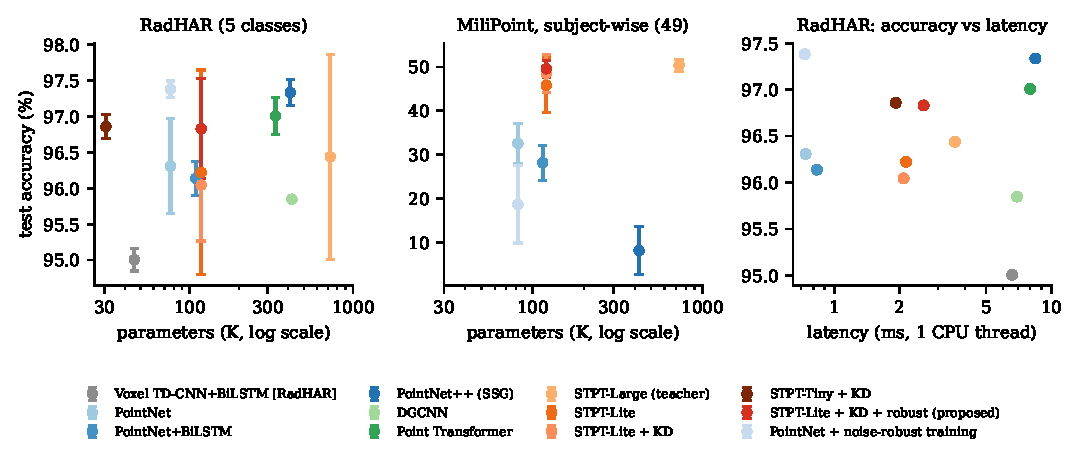
\includegraphics[width=\textwidth]{../figures/efficiency.pdf}
\caption{Accuracy (mean $\pm$ std over seeds) versus parameters on both datasets, and RadHAR accuracy versus single-thread CPU latency.}
\label{fig:efficiency}
\end{figure*}

\subsection{Ablation study}
\label{sec:ablation}
\begin{table}[t]
\centering
\caption{Ablation of STPT-Lite (no distillation): test accuracy (\%), mean\,$\pm$\,std over seeds (variants: 2 on RadHAR, 2 on MiliPoint; full model: 3), change w.r.t.\ the full model trained with the same seeds in brackets; $^\dagger$ single run.}
\label{tab:ablation}
\setlength{\tabcolsep}{3pt}
\resizebox{\columnwidth}{!}{%
\begin{tabular}{lcc}
\toprule
Variant & RadHAR & MiliPoint (subj.) \\
\midrule
STPT-Lite (full, no KD) & 96.22\,$\pm$\,1.43 & 45.79\,$\pm$\,6.30 \\
\midrule
-- intra-segment attention (max+attentive pool only) & 96.90\,$\pm$\,0.18 (+0.93) & 42.87\,$\pm$\,3.03 (-6.52) \\
-- motion descriptor & 97.67\,$\pm$\,0.16 (+1.70) & 49.90\,$\pm$\,2.06 (+0.50) \\
-- temporal Transformer (mean over segments) & 96.70\,$\pm$\,0.61 (+0.73) & 37.54\,$\pm$\,6.62 (-11.85) \\
-- Doppler \& intensity ($xyz$ only) & 96.42\,$\pm$\,1.69 (+0.45) & -- \\
-- spatial gating & 97.62\,$\pm$\,0.40 (+1.64) & -- \\
-- all training augmentation & 96.68\,$\pm$\,0.54 (+0.70) & -- \\
-- coordinate jitter augmentation & 95.86\,$\pm$\,1.13 (-0.11) & -- \\
\bottomrule
\end{tabular}}
\end{table}
Table~\ref{tab:ablation} removes one component of STPT-Lite (without
distillation) at a time and retrains with \ablSeeds{} seeds on RadHAR.
\textbf{MiliPoint (unseen people)} is the informative benchmark for the
architecture. Compared with the full model trained with the same two seeds
(49.4\% on average), removing the temporal Transformer (mean over segment
tokens instead) costs 11.9 points, and removing the intra-segment attention
(pooling only) costs 6.5 points. Both losses hold in each seed separately.
Fine-grained actions are therefore distinguished both by how the returns of a
short segment relate to each other and by how the segments evolve over the
window. The explicit motion descriptor brings no measurable gain (+0.5 points on
average, +2.8 and $-$1.8 in the two seeds): the attention layers apparently
recover centroid and displacement information from the point coordinates
themselves. We keep the descriptor because it costs only 2.5\,K parameters (2\% of the model), but
we do not claim it as a contribution to accuracy. \textbf{RadHAR} cannot rank
components. Every variant, including removing Doppler/intensity, gating or
augmentation, lies within about 1.7 points of the full model, inside its
seed spread ($\pm$1.4), because every model already exceeds 95\%. The
effect of the pre-processing is visible across models instead: with the same gating
and centring, all baselines exceed the published 90.47\%.


\subsection{Evaluation protocol and leakage}
\label{sec:protocol}
\begin{table}[t]
\centering
\caption{MiliPoint (49 actions) top-1 accuracy (\%) of the same models under three splits. Published numbers: 34.45 (PointNet++, \cite{cui2023milipoint}) and 98.25 (MAK-GCN, random 80/10/10, \cite{zakka2025makgcn}).}
\label{tab:protocol}
\setlength{\tabcolsep}{3pt}
\resizebox{\columnwidth}{!}{%
\begin{tabular}{lccc}
\toprule
Model & Subject-disjoint & Chronological & Random windows \\
 & (ours, primary) & (MiliPoint code) & (leaky) \\
\midrule
STPT-Lite & 45.79\,$\pm$\,6.30 & 58.38 (n=1) & 79.48 (n=1) \\
PointNet & 32.57\,$\pm$\,4.59 & 32.42 (n=1) & 44.44 (n=1) \\
\bottomrule
\end{tabular}}
\end{table}
The same STPT-Lite scores \mistptliteAcc\% under our subject-disjoint split,
\mpOfficialAcc\% under the chronological split of the MiliPoint code (which
shares subjects between training and test), and \mpRandomAcc\% under a random
split of overlapping windows (Table~\ref{tab:protocol}). The automated audit
explains this. Under the random split, \mpAuditLeakFrames\% of the test frames
also occur inside training windows, and \mpAuditLeakWins\% of the test windows
overlap a training window, by \mpAuditLeakOverlap\% of their length on average.
The inflation is therefore leakage, not learning. Accuracies of 98\% on
MiliPoint \cite{zakka2025makgcn} and ours of about 50\% describe different
tasks: recognising near-duplicates of seen sequences versus recognising actions
of new people. On RadHAR, the same audit found that every official test
recording lies within ten minutes of a training recording (median gap 29\,s) on
the same four days, and the dataset contains no subject identifiers. RadHAR
accuracy therefore measures generalisation to new recordings of known people
in a known room.

\subsection{Cross-dataset transfer}
\begin{table}[t]
\centering
\caption{Cross-dataset transfer (STPT-Lite, $xyz$ input): test accuracy (\%) when fine-tuning on a fraction of target training recordings/runs, from scratch vs.\ initialised from the model trained on the other dataset (mean\,$\pm$\,std, 3 seeds).}
\label{tab:transfer}
\setlength{\tabcolsep}{3pt}
\resizebox{\columnwidth}{!}{%
\begin{tabular}{llcc}
\toprule
Direction & Target data & Scratch & Pre-trained \\
\midrule
MiliPoint $\rightarrow$ RadHAR & 10\% & -- & -- \\
MiliPoint $\rightarrow$ RadHAR & 25\% & -- & -- \\
MiliPoint $\rightarrow$ RadHAR & 100\% & 95.23\,$\pm$\,0.00 & -- \\
\midrule
RadHAR $\rightarrow$ MiliPoint & 25\% & -- & -- \\
RadHAR $\rightarrow$ MiliPoint & 100\% & 45.79\,$\pm$\,6.30 & -- \\
\bottomrule
\end{tabular}}
\end{table}
Table~\ref{tab:transfer} initialises STPT-Lite from the MiliPoint model ($xyz$
input, harmonised axes) and fine-tunes it on a fraction of the RadHAR training
recordings. Pre-training on MiliPoint helps most when little RadHAR data is available. With
10\% of the RadHAR training recordings it raises test accuracy from
\trrhxyzscratchfTen\% to \trrhxyzmpinitfTen\% (two seeds; +18 points, larger
than the seed spread). With 25\% the gain shrinks to about one point, inside the
seed spread, and with all training data the pre-trained and scratch models are
equivalent (\trrhxyzmpinitfFull\% vs.\ \trrhablxyz\%). Since the two datasets
differ in radar, frame rate, subjects, room and label set, this suggests that
the segment tokenizer learns largely sensor-independent motion features from MiliPoint's
49 actions, which are most valuable when target labels are scarce, as in a new
home with few annotated recordings. With all data, one pre-trained seed reached its best validation score after the
first epoch and was stopped early (93.8\%); we report it unchanged.


\subsection{Noise robustness}
\begin{figure*}[t]
\centering
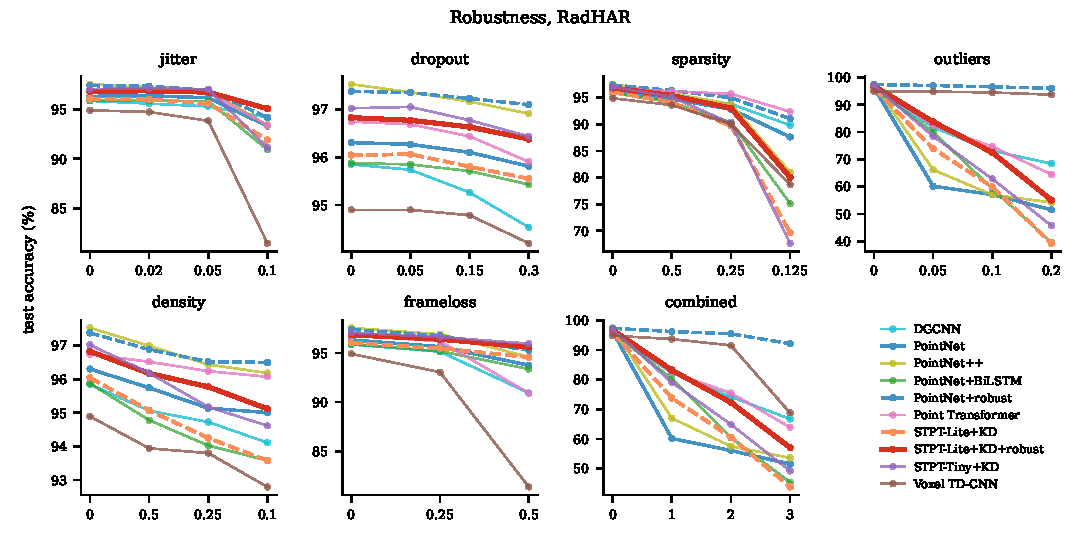
\includegraphics[width=0.49\textwidth]{../figures/robustness_radhar.pdf}\hfill
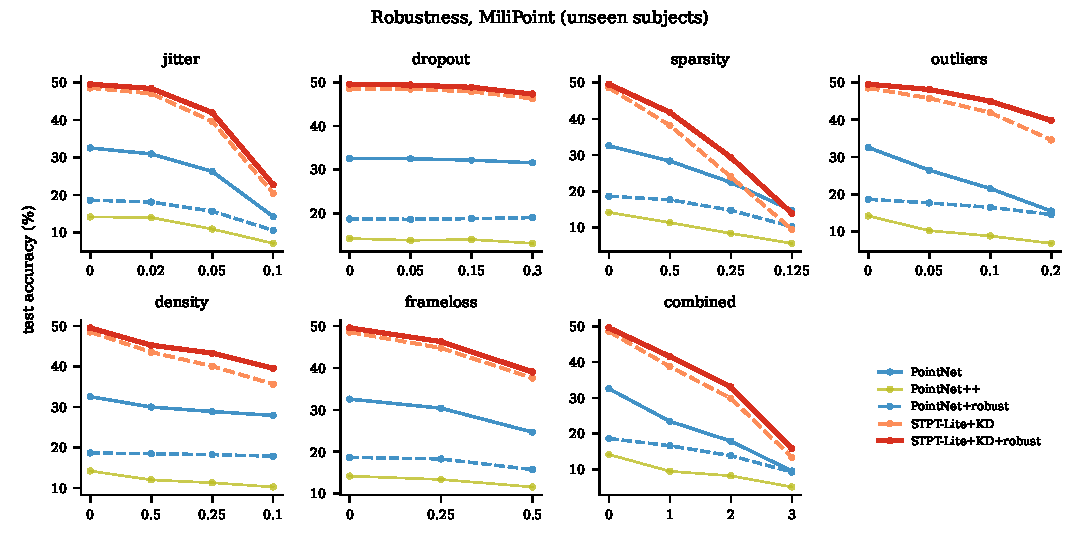
\includegraphics[width=0.49\textwidth]{../figures/robustness_milipoint.pdf}
\caption{Test accuracy under controlled perturbations (identical perturbed samples for every model; mean over the available seeds). Left: RadHAR; right: MiliPoint (unseen subjects).}
\label{fig:robust}
\end{figure*}
Fig.~\ref{fig:robust} reports test accuracy under seven perturbation types,
three severities each, applied with fixed seeds so that every model sees the
same perturbed windows. \textbf{MiliPoint (unseen people).} The proposed model
stays the most accurate under every condition except the most extreme
sparsity. Noise-robust training improves STPT-Lite+KD under all perturbations,
by 0.9--5.4 points (e.g.\ 20\% false detections: 34.6$\rightarrow$39.8\%; density
0.1: 35.6$\rightarrow$39.6\%), including jitter, which was not used in training
(22.8 vs.\ 20.5\% at $\sigma=10$\,cm). At 12.5\% of the returns kept (about one
point per frame), STPT-Lite (13.9\%) falls to the level of PointNet (14.7\%): with
almost no points per segment, intra-segment attention has nothing to attend to.
\textbf{RadHAR.} Dropout, density changes and jitter up to 5\,cm cost every
point-based model at most 2.5 points. Losing half of the segments costs DGCNN and
Point Transformer about five points but the proposed model only 1.2 points
(96.8$\rightarrow$95.6\%), which matches the even temporal attention in
Section~\ref{sec:xai}. Two conditions separate the
models. Under extreme sparsity, Point Transformer (92.4\%) and PointNet with
robust training (91.1\%) degrade least, the proposed model reaches 80.0\%, and
STPT-Lite+KD without robust training drops to 69.7\%. False detections are the
main weakness of the STPT family on RadHAR: at 20\% injected outliers the
proposed model keeps 55.1\% (39.3\% without robust training), whereas PointNet
with the same robust training keeps 96.0\% and the voxel CNN-LSTM 93.7\%.
A likely cause is that outliers corrupt the motion descriptor (centroid, mean Doppler) and receive
attention weight, while a max-pooled PointNet with robust training learns to
ignore isolated points and voxel occupancy dilutes them. Robust training
therefore helps, but it does not close this gap. A robust centroid (median) in
the motion descriptor and outlier-aware attention are the obvious next steps.


\subsection{Explainability and error analysis}
\label{sec:xai}
\begin{figure}[t]
\centering
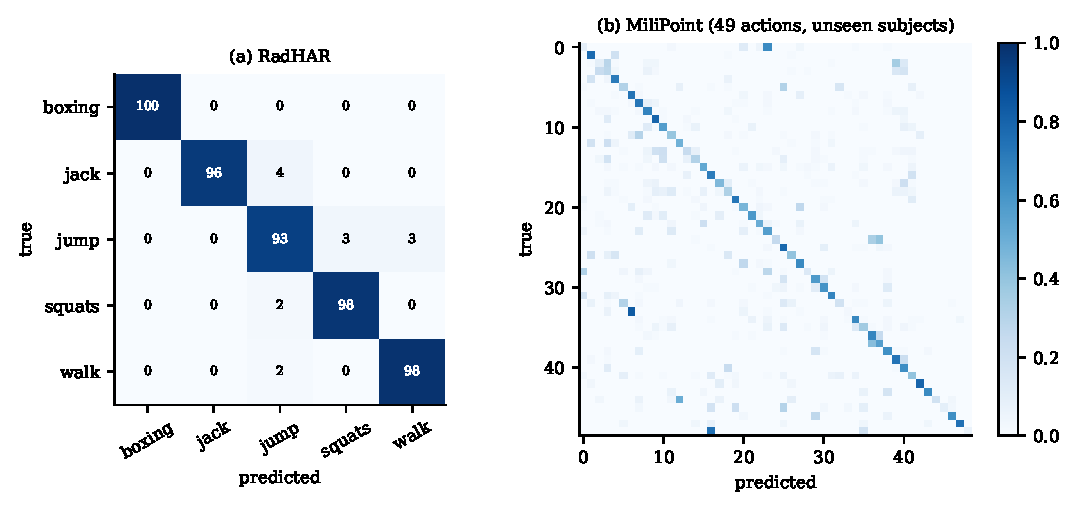
\includegraphics[width=\columnwidth]{../figures/confusion.pdf}
\caption{Row-normalised confusion matrices of the proposed STPT-Lite+KD+robust (seed 0).}
\label{fig:confusion}
\end{figure}
\begin{figure}[t]
\centering
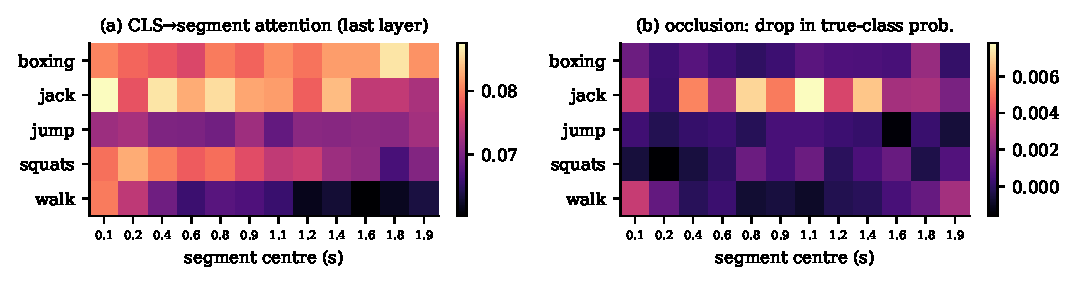
\includegraphics[width=\columnwidth]{../figures/xai_temporal.pdf}
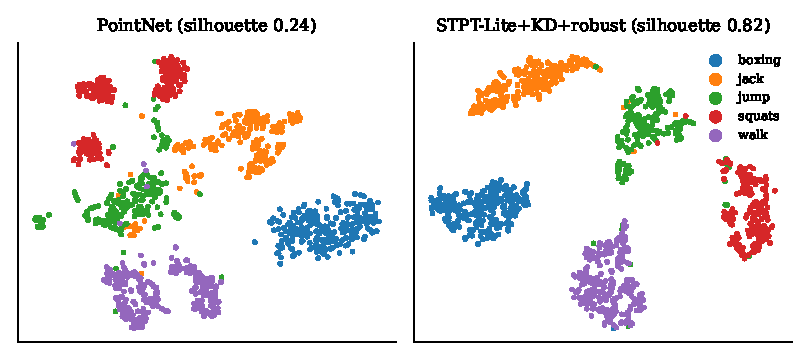
\includegraphics[width=\columnwidth]{../figures/tsne.pdf}
\caption{Top: mean [CLS]$\rightarrow$segment attention and segment-occlusion importance per class (RadHAR test). Bottom: t-SNE of test embeddings.}
\label{fig:xai}
\end{figure}
\textbf{Temporal attention and occlusion.} The [CLS] attention of the last
block is spread almost evenly over the twelve segments (0.07--0.09 per
segment, against 0.083 for uniform attention), with class-specific emphasis: the
middle of the window for jumping jacks, early segments for squats, and the
first segment for walking (Fig.~\ref{fig:xai}). Removing a single segment
(occlusion) lowers the true-class probability by less than one percentage point
on average. The model therefore integrates evidence over the whole window and
does not depend on any single 170-ms segment, which is consistent with its
tolerance to frame loss. Attention and occlusion importance agree only
moderately (Pearson $r=\xaiCorr$ over the class$\times$segment cells), so we
treat attention as a coarse indication and not as a faithful explanation.
\textbf{Point saliency.} Gradient saliency concentrates on the returns of the
moving limbs and torso and is low on isolated returns far from the body,
i.e.\ on the residual clutter that survives gating. \textbf{Embeddings.} In a
t-SNE of RadHAR test embeddings the classes form compact, well-separated
clusters (silhouette \silSTPTLiteKDrobust{} in the model's embedding space
versus \silPointNet{} for PointNet). \textbf{Errors.} The remaining RadHAR
errors are mostly windows predicted as \emph{jump} (precision 91\%), which
shares the strong vertical Doppler pattern of jumping jacks and squats. On
MiliPoint, errors concentrate in groups of kinematically similar actions.


\begin{table}[t]
\centering
\caption{Published results (as reported by the authors, under their own protocols; not directly comparable).}
\label{tab:sota}
\setlength{\tabcolsep}{3pt}
\resizebox{\columnwidth}{!}{%
\begin{tabular}{llrl}
\toprule
Method & Dataset & Acc. (\%) & Protocol / note \\
\midrule
TD-CNN+BiLSTM \cite{singh2019radhar} & RadHAR & 90.47 & official test, window-level val. \\
Lite-PointNet+BiLiLSTM \cite{gu2024lpn} & RadHAR & 95.12 & 79.7\,K params \\
GNN + 3-D joints \cite{lee2022gnn} & RadHAR & 96.55 & joint pre-training \\
MAK-GCN \cite{zakka2025makgcn} & RadHAR & 97.54 & 1.86\,M params \\
OG-PCL \cite{yan2025ogpcl} & RadHAR & 91.75 & 5-fold CV, 0.83\,M params \\
PointNet++ \cite{cui2023milipoint} & MiliPoint & 34.45 & chronological 80/10/10 \\
MAK-GCN \cite{zakka2025makgcn} & MiliPoint & 98.25 & random 80/10/10 \\
\midrule
STPT-Lite+KD+robust (ours) & RadHAR & \rastptlitekdrobustAcc & official test, recording-disjoint val. \\
STPT-Lite+KD+robust (ours) & MiliPoint & \mistptlitekdrobustAcc & subject-disjoint \\
\bottomrule
\end{tabular}}
\end{table}

\textbf{Published results.} Table~\ref{tab:sota} lists accuracies as reported by
other authors. They use different splits, pre-processing and training budgets
and are not directly comparable to ours; we include them for context only.

\section{Limitations}
\textbf{Benchmarks.} RadHAR has two subjects, no subject identifiers, and test
recordings from the same sessions as the training recordings, so it cannot
measure generalisation to new users. MiliPoint offers $xyz$ only and three test
subjects, and its action names are not published. \textbf{Baselines.} All
baselines were re-implemented by us under one training budget (at most 15/30
epochs with early stopping, CPU-only). Our PointNet++ did not train well on
MiliPoint's six-point frames, and DGCNN and Point Transformer were evaluated on
RadHAR only. Published implementations with tuned neighbourhood
parameters and longer training may perform better. \textbf{Robustness.}
Perturbations are applied to recorded point clouds and are not a physical radar
simulation. Under extreme sparsity (12.5\% of returns kept), STPT-Lite falls to
PointNet level on MiliPoint, and on RadHAR it is far more sensitive to injected
false detections than PointNet with the same robust training (55 vs.\ 96\% at
20\% outliers). \textbf{Deployment.} Latency was measured on one desktop CPU
thread, and storage is computed for INT8 weights. On-device deployment was not
performed. \textbf{Scope.} Single person, fixed 2-s windows, no fall labels,
and no clinical validation.

\section{Conclusion and Future Work}
We presented STPT-Lite, a factorised spatio-temporal point transformer for
privacy-preserving activity recognition from sparse mmWave radar point clouds,
together with Doppler-based person centring and clutter gating. On 49 MiliPoint
actions performed by unseen people, the distilled, noise-robust model reaches
\mistptlitekdrobustAcc\% top-1 (\mistptlitekdrobustTopthree\% top-3), about 17 points above the best re-implemented baseline, at
\oursParamsK\,K parameters, \oursMflops\,MFLOPs and \oursLat\,ms per window. On
RadHAR all models saturate at about 95--98\%, and the pre-processing, not the
architecture, explains the gain over the original 90.5\%. A dedicated audit
shows that random window splits leak most test frames into training, which
accounts for much of the spread of published MiliPoint results. Future work:
leave-one-subject-out and cross-room evaluation on datasets with subject
identifiers and fall events, deployment on the radar's companion processor, and
self-supervised pre-training on the large unlabelled portions of both datasets.


\section*{Acknowledgment}
We thank the faculty of the Department of Information Technology, PSG College of
Technology, for their guidance during the 23I006 Deep Learning course, and the
authors of RadHAR and MiliPoint for releasing their datasets.

\bibliographystyle{IEEEtran}
\bibliography{refs}

\end{document}
